\section{系统实现}
\subsection{系统实现环境}
树莓派、2T西部数据机械硬盘、机械硬盘电源、500Mb/s网卡速率TP-Link路由器
\subsection{系统功能实现}

\subsubsection{用户登录}
登录注册需要一个很长的验证过程,下面的流程图给出很了很详细的验证过程。登录注册的流程图是功能需求分析的时候开始设计,考虑了很多因素进去,
包括了更重成功、失败结果如何进行处理。但是因为开发时间紧迫,目前本系统只实现了用户名,口令登录部分,剩下的部分在之后的完善计划中会有进一步
的工作。

因为本系统Web端和安卓转都使用同一的接口进行登录,所以服务器会返回一个同一的requesttoken作为身份验证。传统的浏览器登录方案中,是浏览器发送的
登录请求在服务器验证通过之后,服务器发回SESSIONID和重定向地址,浏览器会自动将SESSIONID地存入Cookie中作为下次请求的身份验证。服务器端会
使用基于动态代理实现的面向切面编程的思想对所有请求进行拦截做身份验证,一般服务器会在SESSION中存有登录成功后的用户信息,服务器端的SESSION
相当于一张hash表,根据客户端请求头中cookie值来判断SESSION中是否保存有用户信息,如果没有,那么就说明发送请求的客户端处于非登录状态,
那么服务器就会发回402代码,如果存在用户信息,那么就会将客户端请求放行。

\begin{figure}[H]
  \centering
  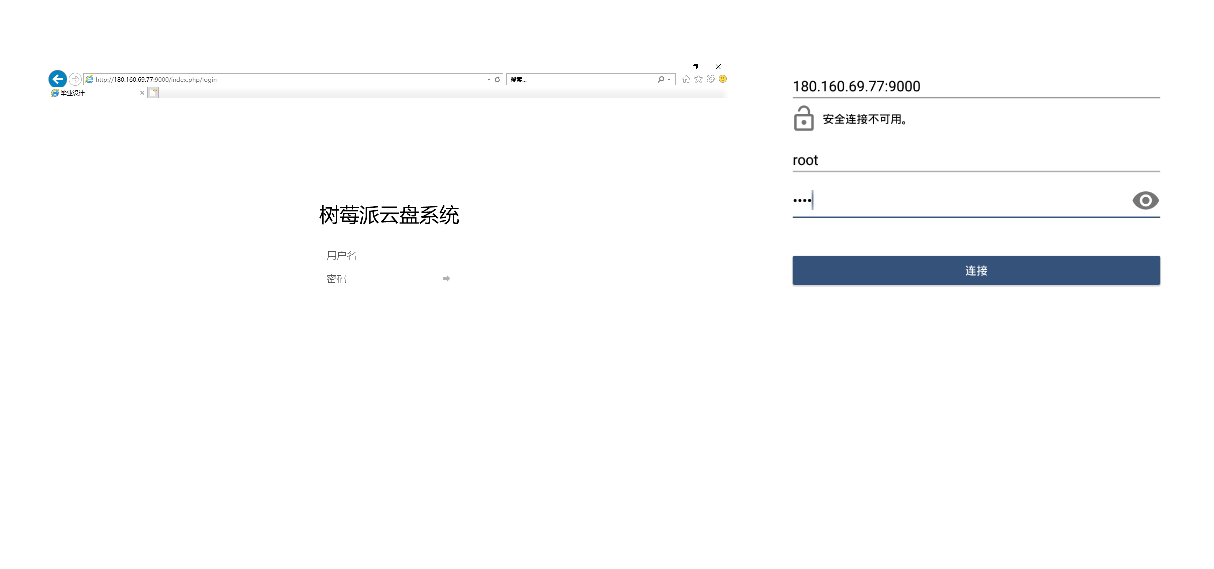
\includegraphics[width=130mm]{./figures/android_web_login.png}
  \caption{安卓、网页登录界面}
\end{figure}

不同于传统的登录实现方案,本系统存在安卓客户端和web客户端,为了避免写两套接口实现一样的功能从而带来开发效率的降低,服务器采用restful的
思想统一web客户端和安卓客户端的接口。所以本系统的登录验证过程是这样的,客户端发送登录初始请求,服务端生成requesttoken并保存在SESSION中,
并返回requesttoken,在web端,浏览器会把requesttoken写入Cookie中。安卓端的网络层使用Retrofit2 + RxJava + Okhttp3框架,安卓端在接收到
requesttoken后,会对requesttoken进行持久化处理,然后当每次使用Retrofit发送请求时,就会在Retrofit请求头中加入requettoken的头部信息,从而
达到身份验证的效果。
\begin{figure}[H]
  \centering
  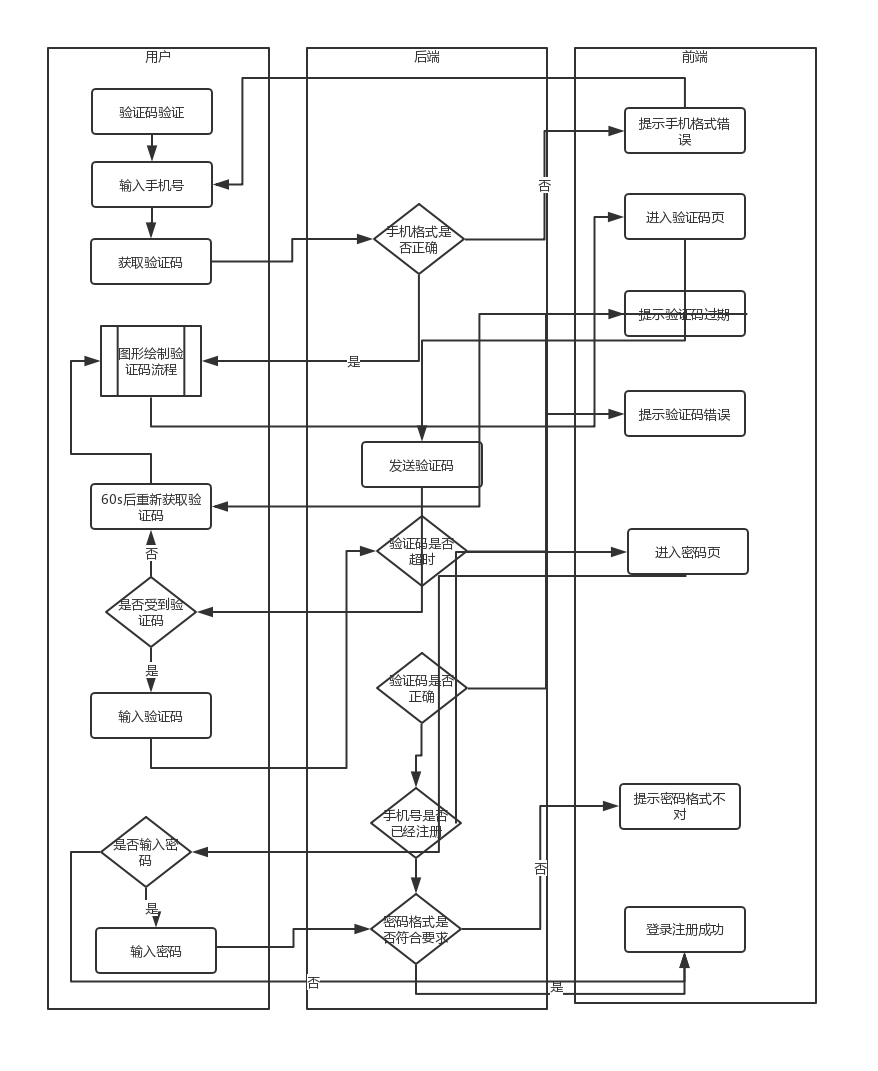
\includegraphics[width=130mm]{./figures/login_liucheng.png}
  \caption{登录注册流程}
\end{figure}

\subsubsection{文件上传}
要保证大文件上传下载的完整性,就需要断点续传的解决方案。

基本的思路是基于阻塞队列BlockingQueue使用生产者消费者模式,
开启读文件线程将大文件切割成固定大小的part,读取后存入阻塞队列BlockinQueue中,
同时开启上传线程将BlockingQueue中part上传。
BlockinQueue为固定大小,在本系统中设置为cpu的核心数4,如果BlockingQueue中
的part数量大于BlockingQueue容量,则读文件线程陷入阻塞状态,如果BlockingQueue为空,
则上传进程陷入阻塞状态,同时,如果读文件读完文件,会将NULL值加入BlockingQueue中,
当上传线程读到NULL时,代表所有文件块已经全部上传,这时会通知服务器对文件进行合并\cite{r30}。

下面给出了本系统使用多线程断点下载的流程图。
\begin{figure}[H]
  \centering
  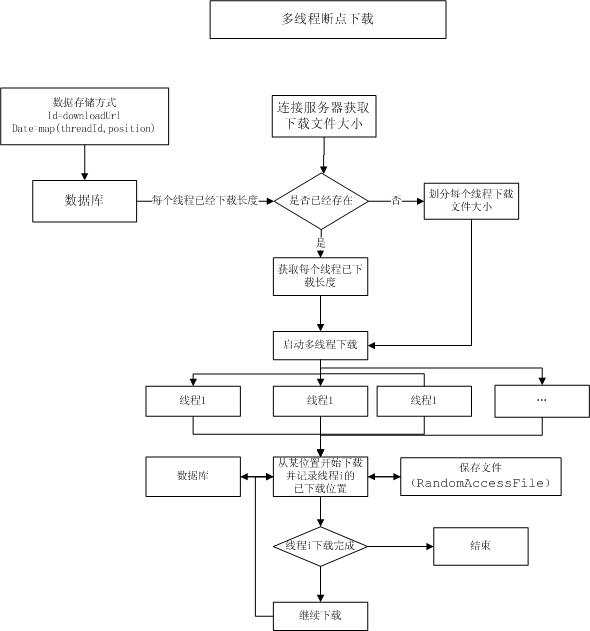
\includegraphics[width=130mm]{./figures/duandian.jpg}
  \caption{断点续传下载实现}
\end{figure}
本系统提供web端和安卓进行文件上传。

\par 安卓可以选择特定目录文件、及时拍照图片、最近修改图片进行上传。同时服务器会对上传文件加锁,如果上传的过程中
用一个并发的线程上传相同路径下的相同文件名文件,那么改线程就会陷入等待轮询状态。如果发现上传的文件有相同文件名,
那么就会提示是否覆盖,如果用户选择不覆盖原有文件,系统会为新文件添加序列号来保证相同路径下文件名的唯一性。
\begin{figure}[H]
    \centering
    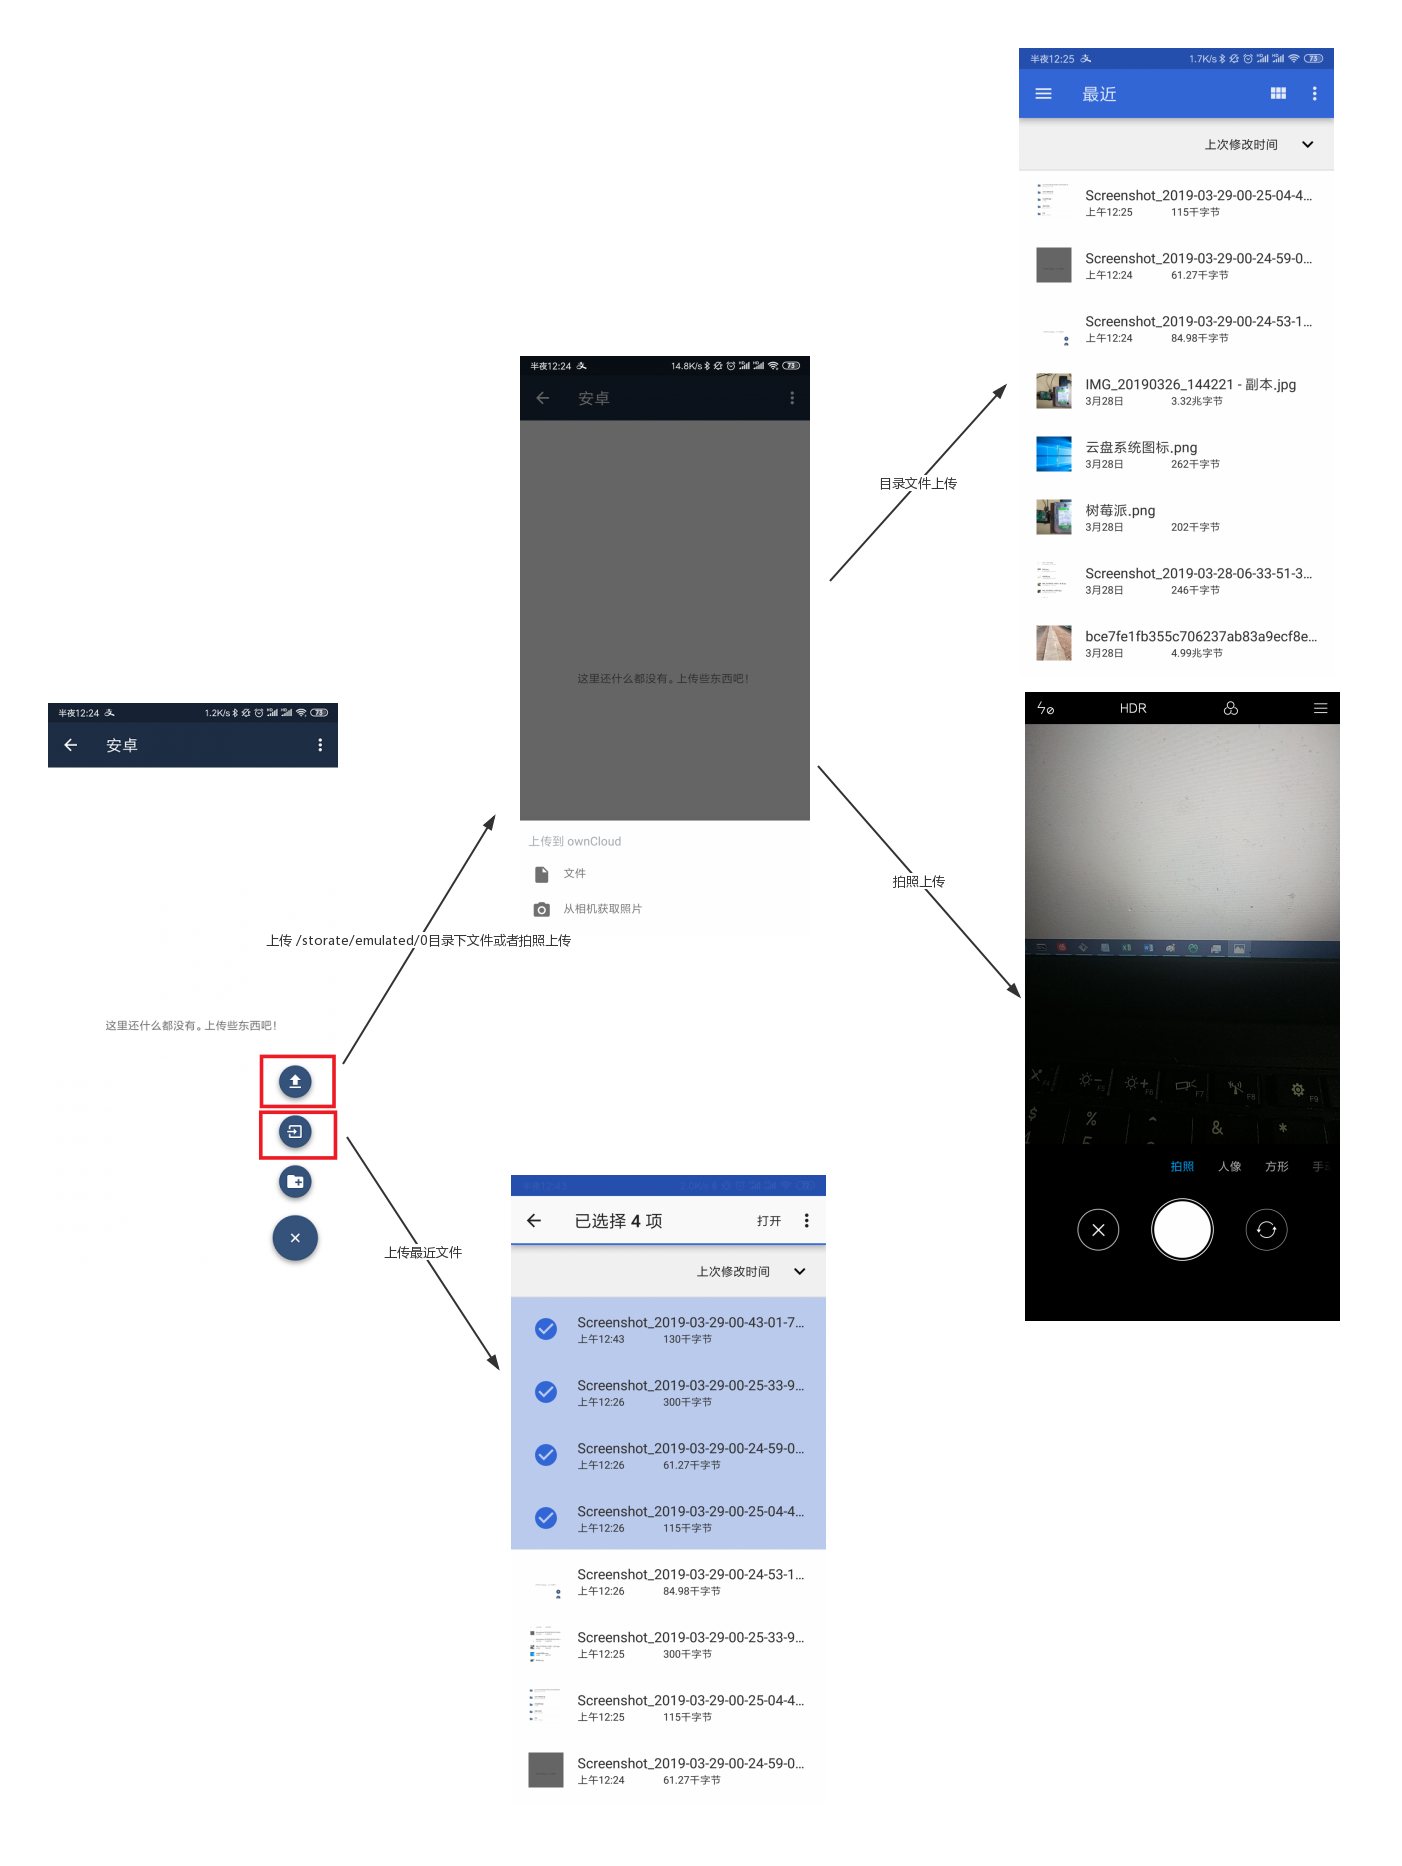
\includegraphics[width=130mm]{./figures/android_file_upload.png}
    \caption{安卓文件上传}
  \end{figure}
\subsubsection{文件下载}
\begin{figure}[H]
    \centering
    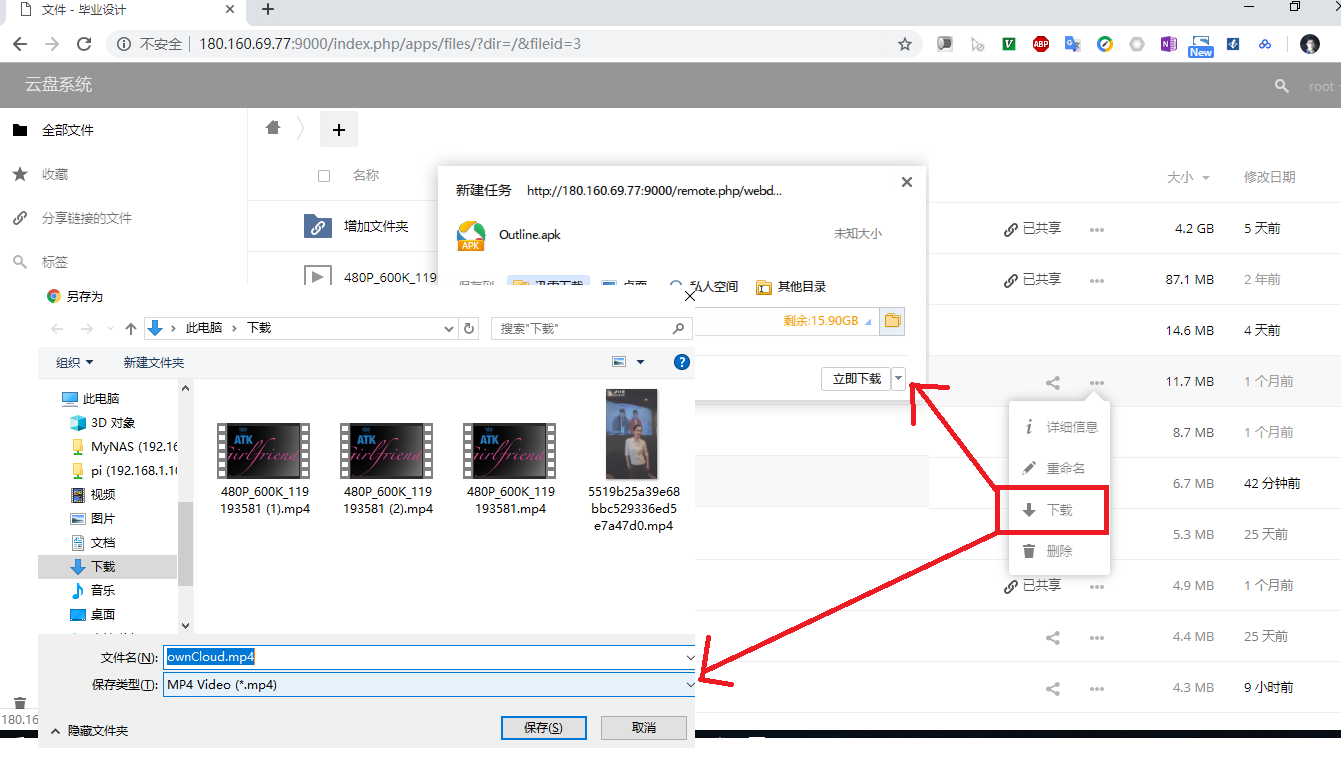
\includegraphics[width=130mm]{./figures/web_file_download.png}
    \caption{网页文件下载}
  \end{figure}

\subsubsection{视频播放}web端和Android端都支持视频播放功能,用户可以在线观看视频,web端视频播放器基于html5的videos标签,可以直接访问在apache
上的静态资源,省去了搭建流媒体服务器的麻烦。
\begin{figure}[htbp]
  \centering
  \subfigure[web在线视频播放器]{
  \begin{minipage}[t]{0.75\linewidth}
  \centering
  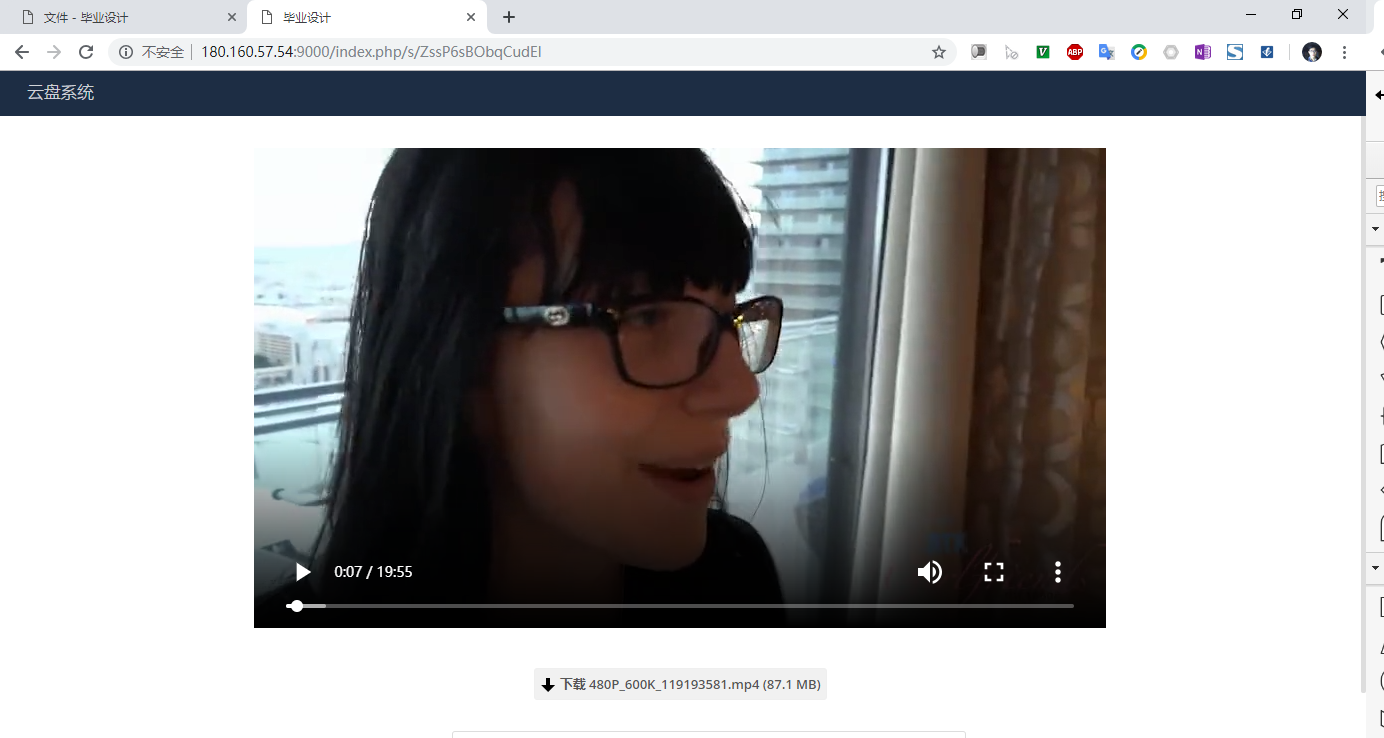
\includegraphics[width=98mm]{./figures/web_videos.png}
  %\caption{fig1}
  \end{minipage}%
  }%
  \subfigure[Android在线视频播放器]{
  \begin{minipage}[t]{0.25\linewidth}
  \centering
  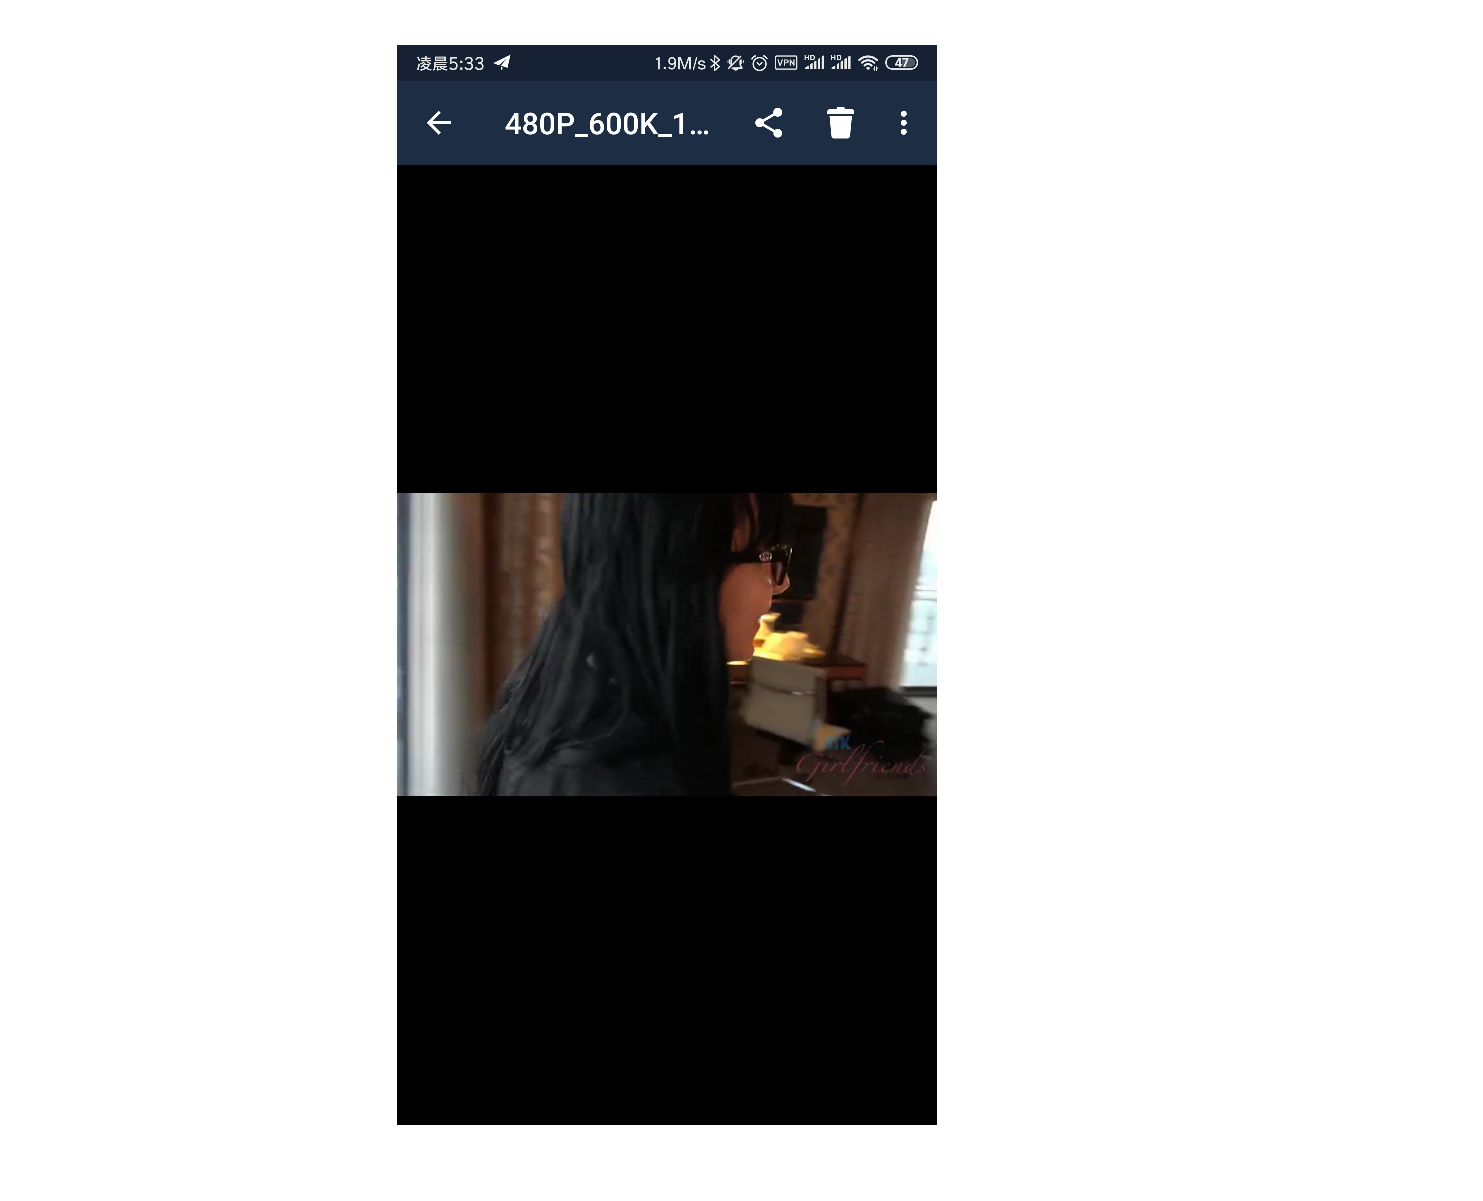
\includegraphics[width=32mm]{./figures/android_videos.png}
  %\caption{fig2}
  \end{minipage}%
  }%
  \centering
  \caption{视频播放}
  \end{figure}
  
\subsubsection{文件分享}
用户点击创建公共链接,客户端发送请求给服务器,服务器首先判断公共链接是否已经创建,如果已经创建,则返回已创建链接,
否则,利用php的shuffle随机函数根据文件uuid生成随机字符存入数据库并返回客户端。客户单端根据返回信息对连接名称,
分享密码,过期时间进行初始化,用户可以修改链接名称、密码、过期日期等信息,发送回服务器,服务器将请求参数持久化到mysql
数据库。

生成分享连接后,用户可以手动复制,通过社交软件或者邮件分享给互联网上的所有用户。安卓端有提供分享接口,通过实现
系统接口可以调用包括QQ、微信、短信、电子邮件或者其他第三发应用进行文件分享。
\begin{figure}[H]
    \centering
    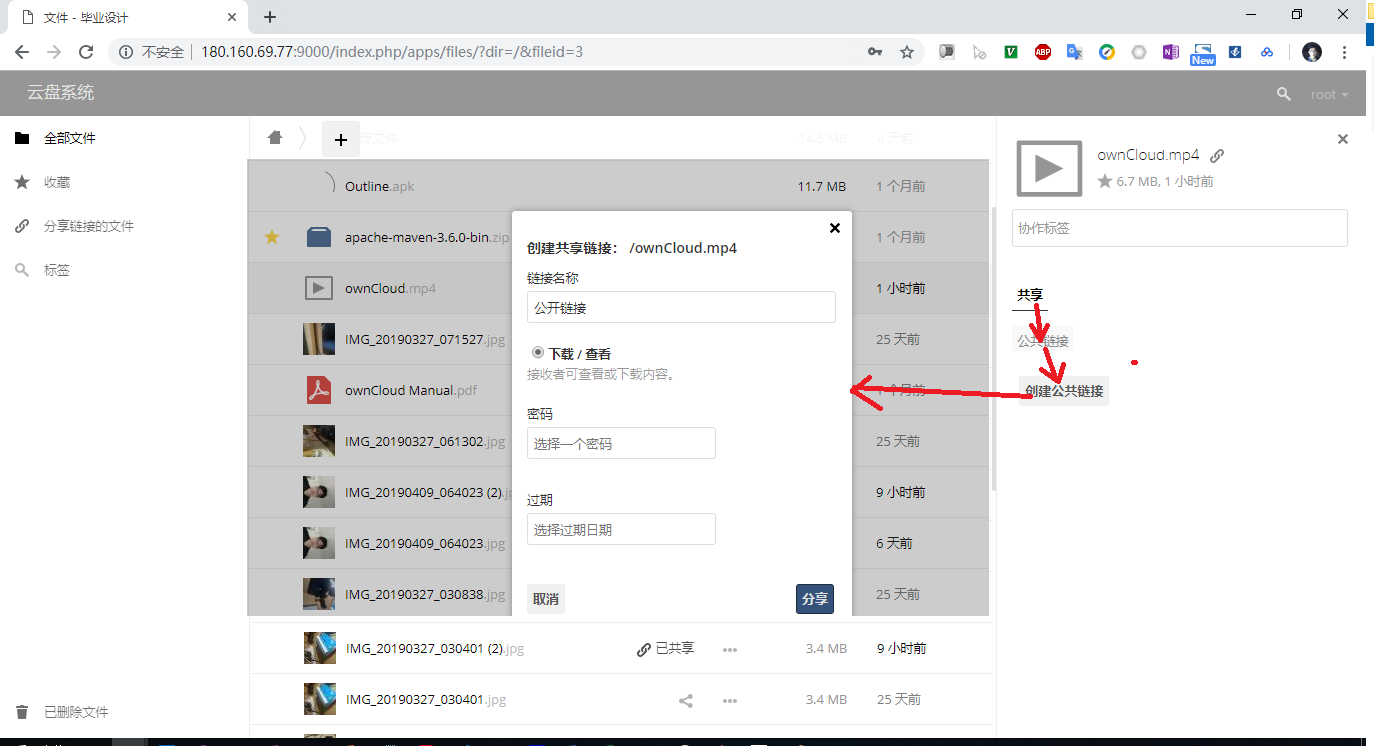
\includegraphics[width=130mm]{./figures/web_file_share_1.png}
    \caption{web分享文件}
    \label{android_videos}
  \end{figure}
\begin{figure}[H]
\centering
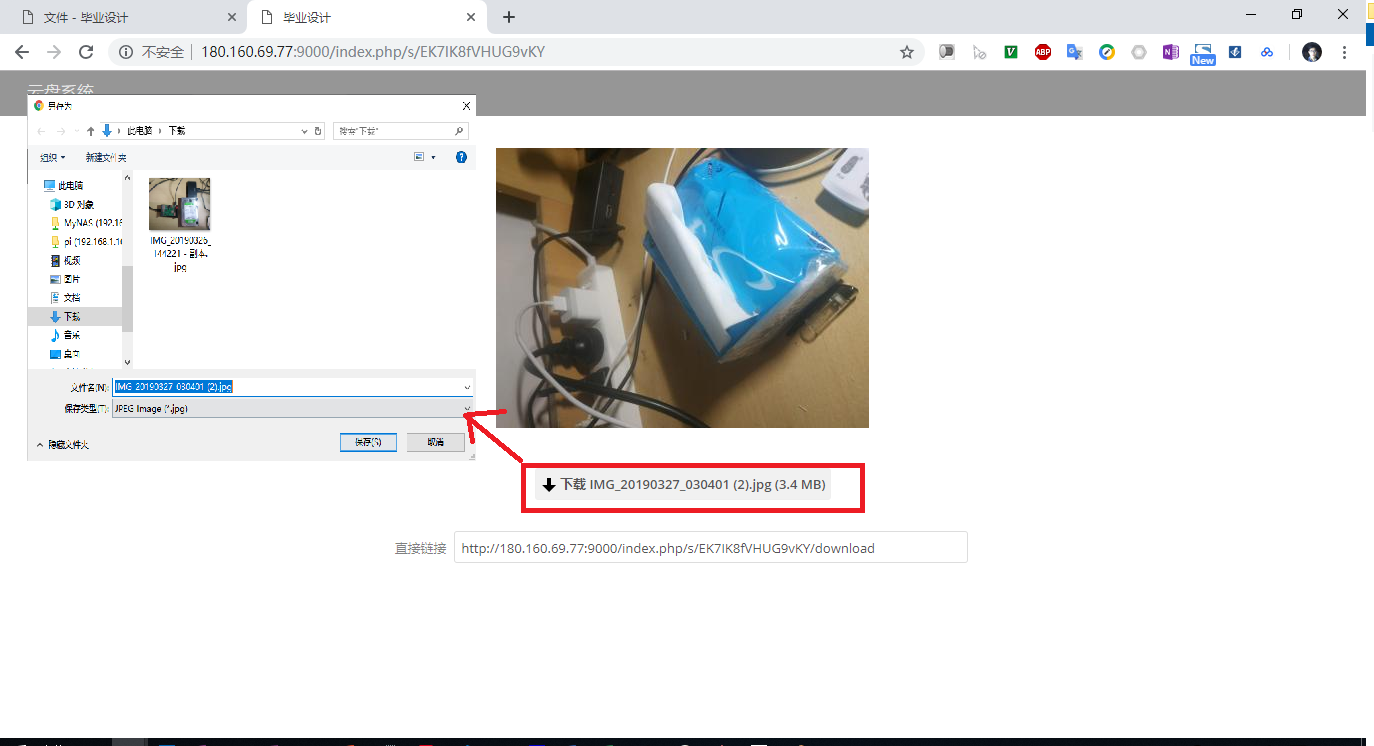
\includegraphics[width=130mm]{./figures/web_file_share_2.png}
\caption{web端访问分享文件}
\label{android_videos}
\end{figure}

\begin{figure}[H]
    \centering
    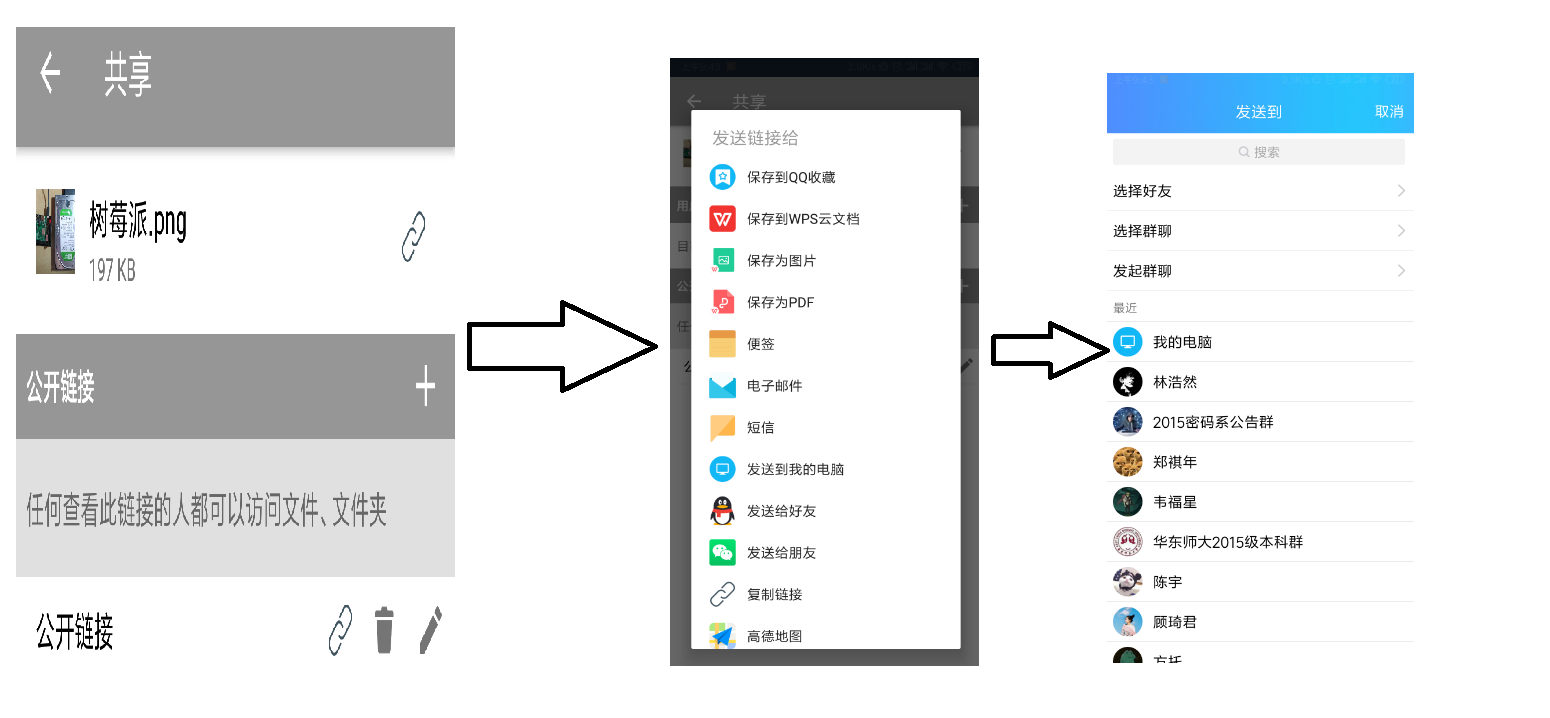
\includegraphics[width=130mm]{./figures/android_file_share.png}
    \caption{安卓端分享文件}
    \label{android_videos}
  \end{figure}

\subsubsection{手机文件自动备份}
安卓客户端默认不提供自动备份功能,因为自动备份的实现是安卓客户端会在后台开启一个backup的service线程,然后
以固定的时间轮询查看备份目录是否用新文件增加,如果用增加,service会调用volley网络请求工具上传文件给服务器,
并在本地保存上传快照。

用户也可以选择是仅上传图片、仅上传视频、仅WiFi网络条件下上传、上传文件后是否保留原文件等设置项。
\begin{figure}[H]
    \centering
    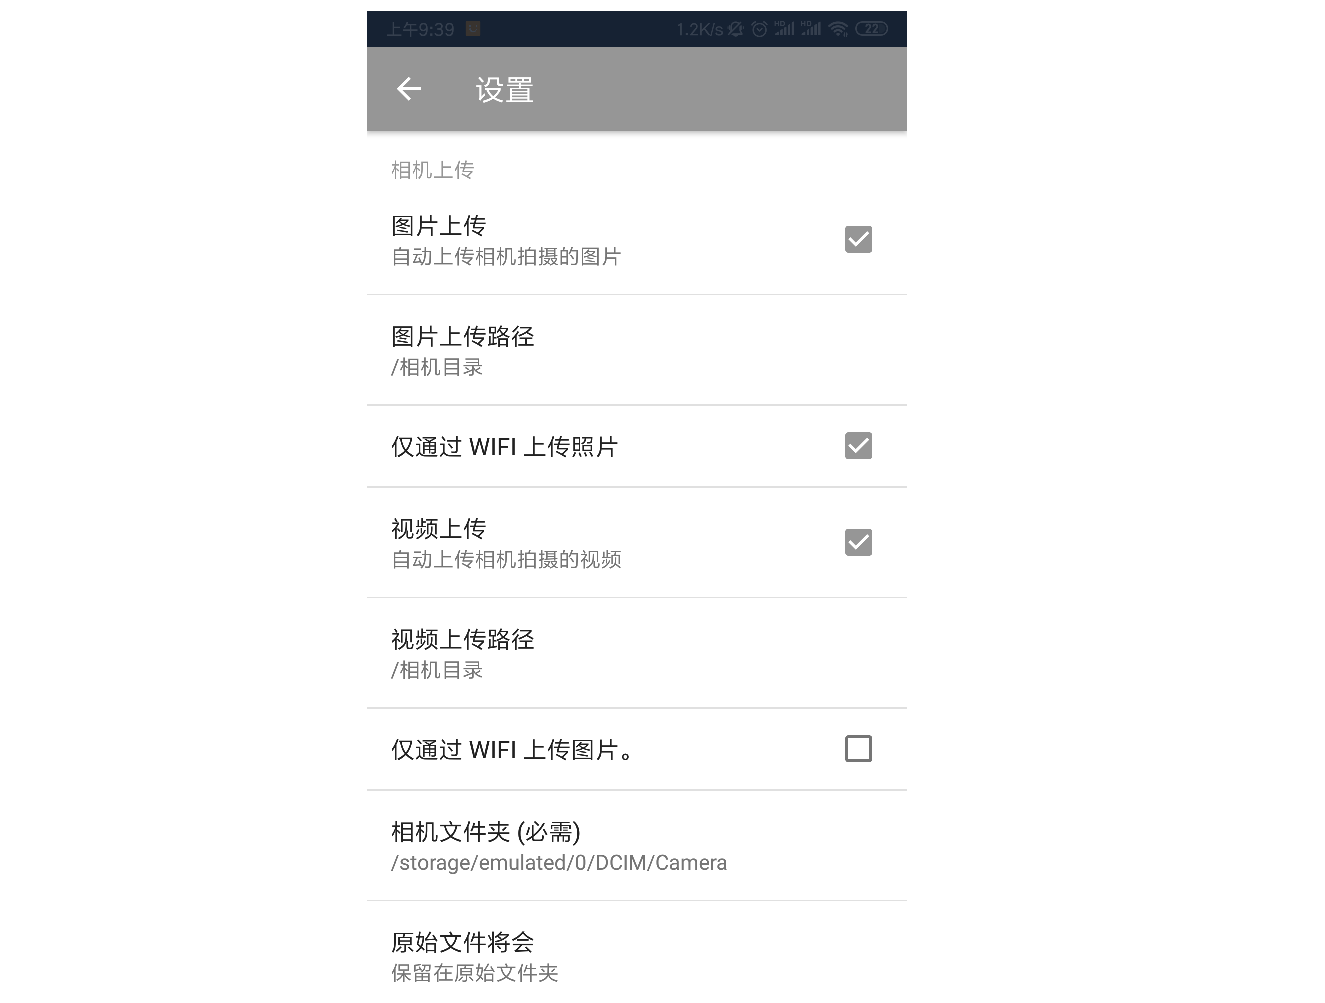
\includegraphics[width=130mm]{./figures/android_file_bck.png}
    \caption{安卓端文件备份设置}
    \label{android_videos}
  \end{figure}

\subsubsection{文件收藏、标签、搜索、已删除文件分类实现}
系统会将文件分为全部文件、收藏、分享文件、已删除文件四大类,用户可以根据自己的需求为文件分类或者打标签,
在web客户端会提供不通文件类型的入口,极大方便了用户查找文件。

实现的原理是创建四张文件表,用户在为文件归类时会往数据表中写入数据,所有文件默认时全部文件类型。当用户进入不同
的文件入口时,服务器会各自查询MySQL中的数据表,返回结果会客户端。
\begin{figure}[H]
    \centering
    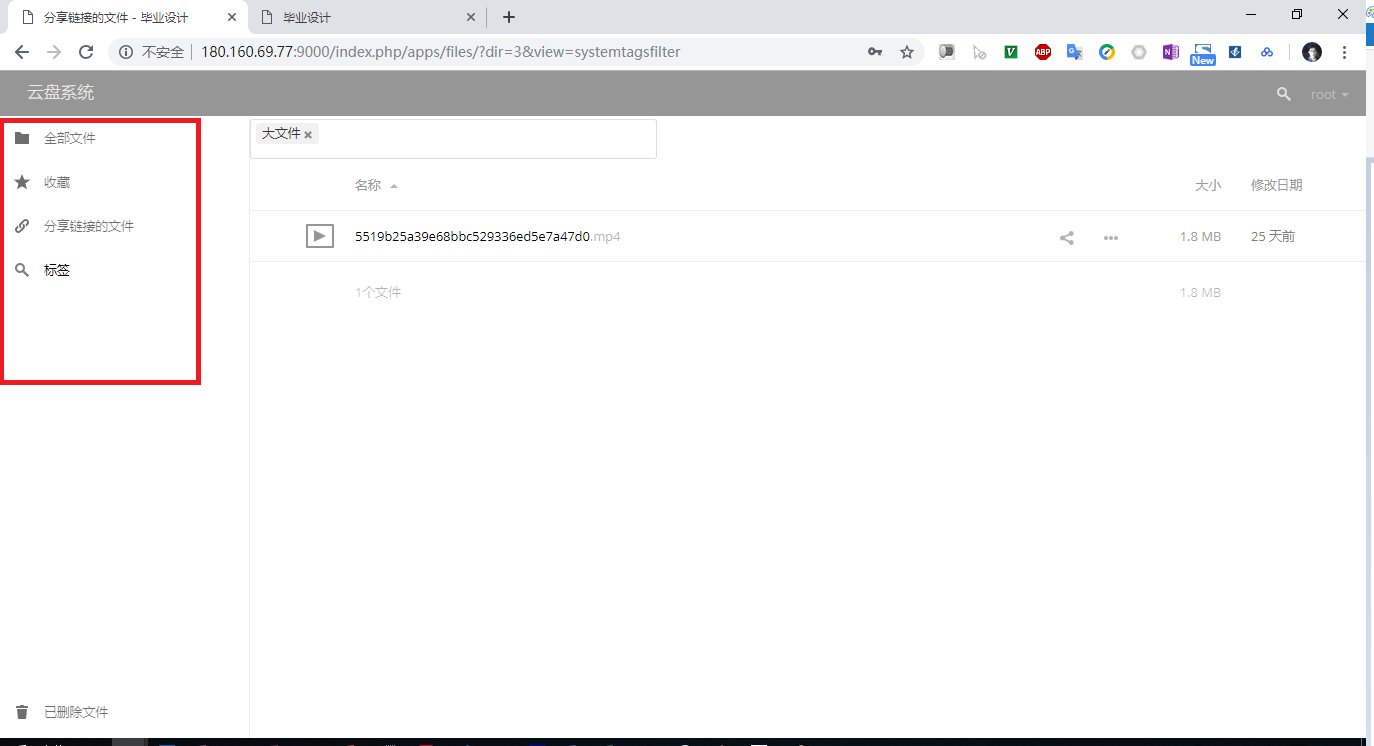
\includegraphics[width=130mm]{./figures/web_file_attach.png}
    \caption{安卓端文件备份设置}
    \label{android_videos}s
  \end{figure}

\subsubsection{文件增量备份、异地备份实现}
Merkle树是一种基于哈希的数据结构。 Merkle树是树状数据结构,其中树中的每个叶节点是数据块,
并且每个非叶节点是其子节点组合的散列。 通常,Merkle树是二叉树,这意味着Merkle树中的每个节点都有两
个子节点。 当然,Merkle树可以是多叉树,例如以太坊平台。 为简单起见,我们将在本文中仅讨论二进制Merkle树。

Merkle树广泛用于分布式系统中进行数据验证\cite{r20,r21}。 通常在分布式系统中,由于我们将数据存储在许多不同的机器上,
因此数据验证对于确保数据的可靠性和一致性尤为重要。 例如,如果我们更新机器上的一段数据,
则必须将更新传递给分布式系统中的所有机器以确保数据的最终一致性,以便比较不同机器上的数据。
\begin{figure}[H]
    \centering
    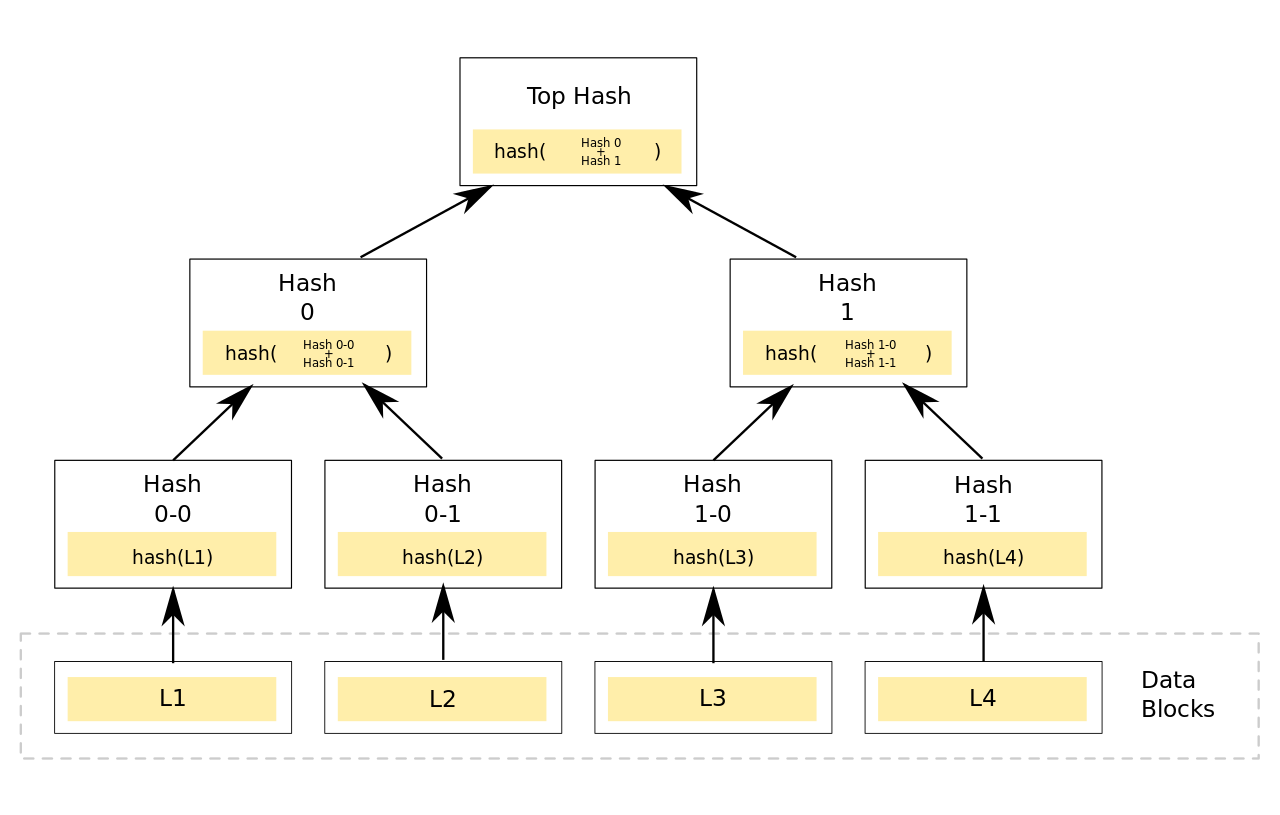
\includegraphics[width=130mm]{./figures/merkle_tree.png}
    \caption{Merkel树}
    \label{android_videos}s
  \end{figure}

本系统至少需要两台服务器进行数据备份,服务器间的数据必须保持同步。 如果数据不一致,则必须快速定位不一致的节点。
本系统为每台机器上的每个目录实现Merkle树,以便在比较两台机器之间的数据时,可以从Merkle树
根节点开始比较。 如果根节点相同,则表示两个副本当前一致,不再需要任何处理; 如果不一致,则遍历Merkle树,
可以快速定位到不一致的节点进行备份。相比于无脑地对文件进行完全备份,使用文件的哈希值作为文件的身份标识来
构建Merkle树的做法提升了备份的速度和存储空间

文件备份流程
\par (1) A服务器向B服务器发送需要与Merkle树的根节点对应的哈希值。
\par (2) B服务器接收此值并将其与正在构建的Merkle树的根节点哈希进行比较。
\par (3) 如果两个值相同,则表示两者存储的文件相同。
\par (4) 否则,B服务器需要像A服务器那样的哈希值来请求与根节点对应的两个子节点。
\par (5) A服务器将相应的值发送给B服务器。
\par (6) B服务器比较相应节点中的散列值,并重复步骤4和5,直到B服务器找到导致不同散列值的一个或多个数据块。
